\chapter{Técnicas de Diseño}\label{sec-patrones}

\section{Patrones de Diseño}
``Un patrón describe un problema recurrente sobre un ambiente, y entonces describe la técnica que soluciona el problema de forma tal que puede ser utilizado sobre cualquier instancia del problema''\cite{DesignPatterns}, es decir, que dados los requerimientos funcionales del sistema es posible analizar la comunicación entre sus distintas partes y de esta forma saber lo patrones que son útiles para dar solución. Los patrones son organizados en tres categorías\cite{DesignPatterns}:
\begin{itemize}
	\item \textbf{Creacionales}: describen la forma en que las entidades (objetos si se utiliza el paradigma orientado a objetos) del sistema son creadas.
	\item \textbf{Estructurales}: describen la organización entre las entidades del sistema.
	\item \textbf{Comportamiento}: describen la comunicación entre entidades del sistema
\end{itemize}

\section{Patrón Singleton}\label{sec-singleton}
El patrón Singleton pertenece al grupo de patrones de diseño de creación, es una forma de proporcionar acceso global a la instancia de una clase sin dar acceso al constructor de la clase y además garantizar que dicha instancia sea la única de la clase. El patrón Singleton identifica principalmente una clase, la cual es encargada de encapsular la creación de su instancia y proveer acceso a dicha instancia\cite{DesignPatternsLasater, DesignPatterns, OCPJavaSE7}.

\begin{figure}[h]
  \centering
  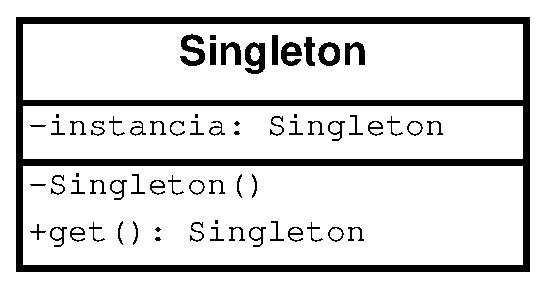
\includegraphics[scale=0.4]{dia-class-singleton}
  \caption{Diagrama UML del patrón Singleton\cite{DesignPatternsLasater}.}
  \label{fig:dia-class-singleton}
\end{figure}

\section{Patrón Strategy}\label{sec-strategy}
El patrón de diseño Strategy es un patrón de diseño de comportamiento, es un grupo de algoritmos encapsulados en clases específicas que pueden ser intercambiadas de modo tal que dependiendo del uso específico se selecciona la clase adecuada. El patrón Stratetegy expone una clase llamada contexto mediante la cual se tiene acceso a las clases con estrategías espíficas que implementan una misma interfaz como se muestra en la Figura \ref{fig:dia-class-strategy} \cite{DesignPatternsLasater, DesignPatterns}.

\begin{figure}[h]
  \centering
  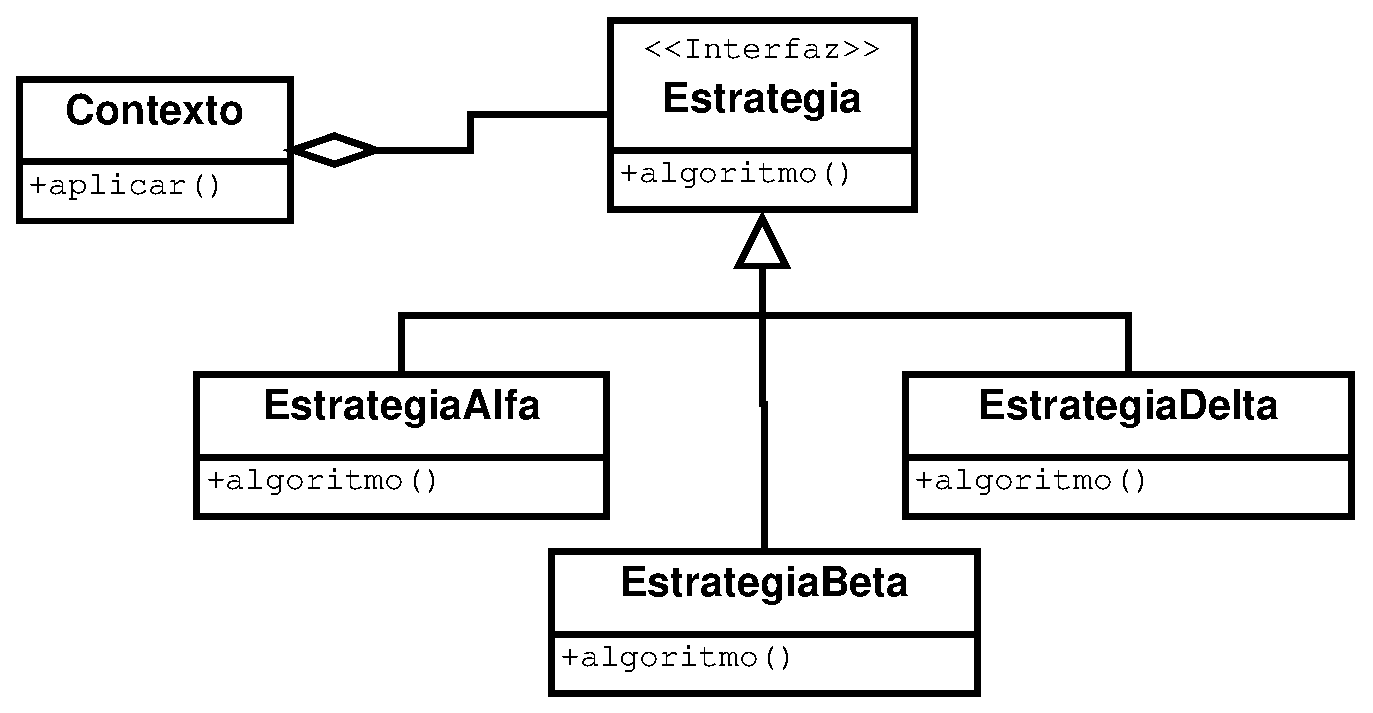
\includegraphics[scale=0.4]{dia-class-strategy}
  \caption{Diagrama UML del patrón Strategy\cite{DesignPatternsLasater}.}
  \label{fig:dia-class-strategy}
\end{figure}

\section{Patrón Decorador}\label{sec-decorator}
El patrón Decorador es utilizado para agregar comportamiento adicional a una clase, tiene cuatro partes principales\cite{DesignPatternsLasater} (ver Figura \ref{fig:dia-class-decorator}):
\begin{enumerate}
  \item Componente: es una clase abstracta que contiene la funcionalidad básica para las clases no decoradas y las decoradas.
  \item Componente concreto: es la implementación de la clase Componente.
  \item Decorador: esta clase es hija de la clase Componente y envuelve una instancias del Componente concreto.
  \item Decorador concreto: es la implementación de la clase que agrega la funcionalidad a la instancia de la clase Componente.
\end{enumerate}

\begin{figure}[h]
  \centering
  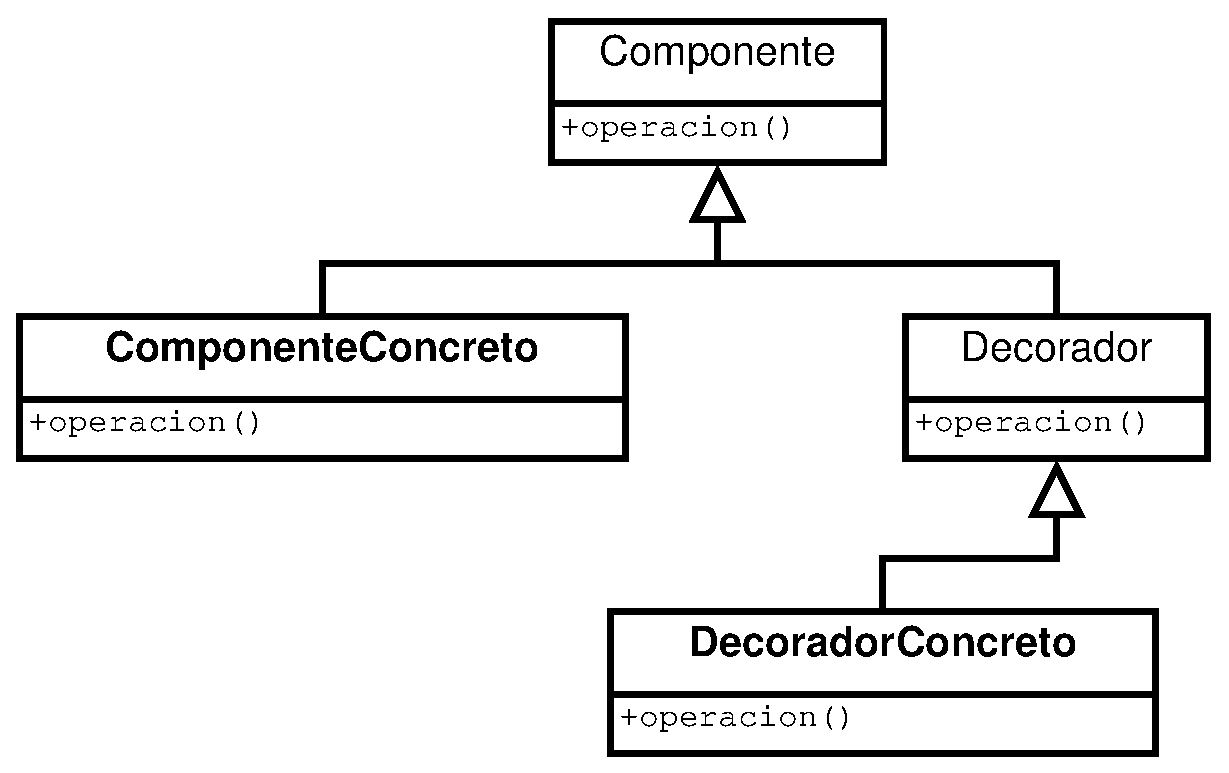
\includegraphics[scale=0.4]{dia-class-decorator}
  \caption{Diagrama UML del patrón Decorador\cite{DesignPatternsLasater}.}
  \label{fig:dia-class-decorator}
\end{figure}

\section{Patrón Proxy}\label{sec-proxy}
El patrón Proxy es una clase que actuá como punto de acceso a otra clase la cual tiene la funcionalidad deseada por algún cliente\cite{DesignPatternsLasater} (ver Figura \ref{fig:dia-class-proxy}):
\begin{enumerate}
  \item Tema: define una interfaz en común para el Tema real y el Proxy.
  \item Tema real: es la clase concreta que representa el Proxy.
  \item Proxy: mantiene referencia a una instancia de la clase Tema real y actúa como punto de acceso a la misma clase.
\end{enumerate}
\begin{figure}[h]
  \centering
  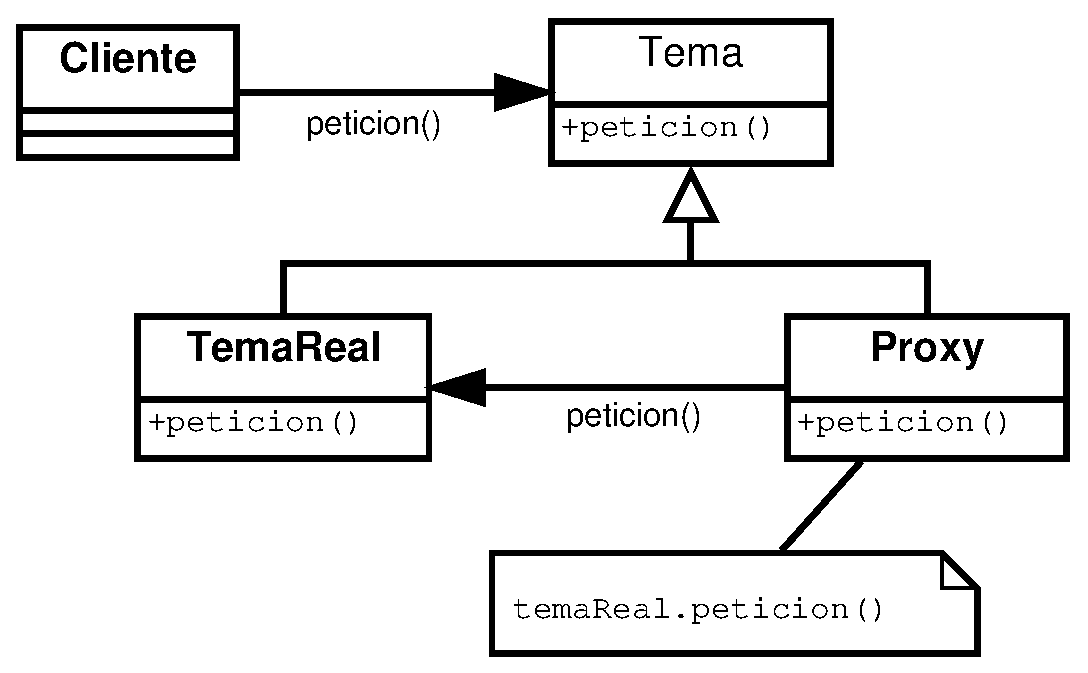
\includegraphics[scale=0.4]{dia-class-proxy}
  \caption{Diagrama UML del patrón Proxy\cite{DesignPatternsLasater}.}
  \label{fig:dia-class-proxy}
\end{figure}

\section{Patrón Objeto de Acceso a Datos}\label{sec-dao}
El patrón Objeto de Acceso a Datos (DAO por sus siglas en inglés) encapsula y abstrae la conexión a una fuente de datos (archivos de texto plano, bases de datos relacionales, bases de datos no relacionales, etc.) y expone operaciones pertinentes al manejo de tales datos\cite{OCPJavaSE7,OCAPJavaSE7}:
\begin{enumerate}
	\item [] \textbf{buscar}: realiza la búsqueda de un único elemento, en caso de no encontrarse tal elemento la respuesta es nula.
	\item [] \textbf{listar}: extrae todos los elementos, el resultado puede utilizar estrategias de paginación.
	\item [] \textbf{insertar}: guarda un nuevo elemento en la fuente de datos.
	\item [] \textbf{actualizar}: actualiza la información de un elemento existente en la fuente de datos.
	\item [] \textbf{borrar}: borra el registro de un elemento en la fuente de datos.
\end{enumerate}


\section{Patrón Modelo-Vista-Controlador}\label{sec-mvc}
Para Sarcar\cite{JavaDesignPatternsExamples} el patrón Modelo Vista Controlador (MVC) es un patrón de arquitectura que consiste de tres grandes componentes: Modelo, Vista y Controlador. El Controlador conduce la comunicación entre la Vista y el Modelo, en la Figura \ref{fig:dia-mvc-simple} se muestra el flujo de comunicación entre los componentes MVC.
\begin{enumerate}
	\item \textbf{Modelo}: tiene la responsabilidad de manejar el acceso a los datos persistentes y la lógica de negocio, usualmente se acompaña del patrón DAO (ver sección \ref{sec-dao}) para el manejo de datos.
	\item \textbf{Vista}: es la capa de presentación, es responsable de mostrar los datos al actor\footnote{Puede ser una persona u otro sistema} que use el sistema.
	\item \textbf{Controlador}: es el intermediario entre la Vista y el Modelo: comunica las peticiones de la vista al modelo y los datos del modelo a la vista.
\end{enumerate}
\begin{figure}[h]
  \centering
  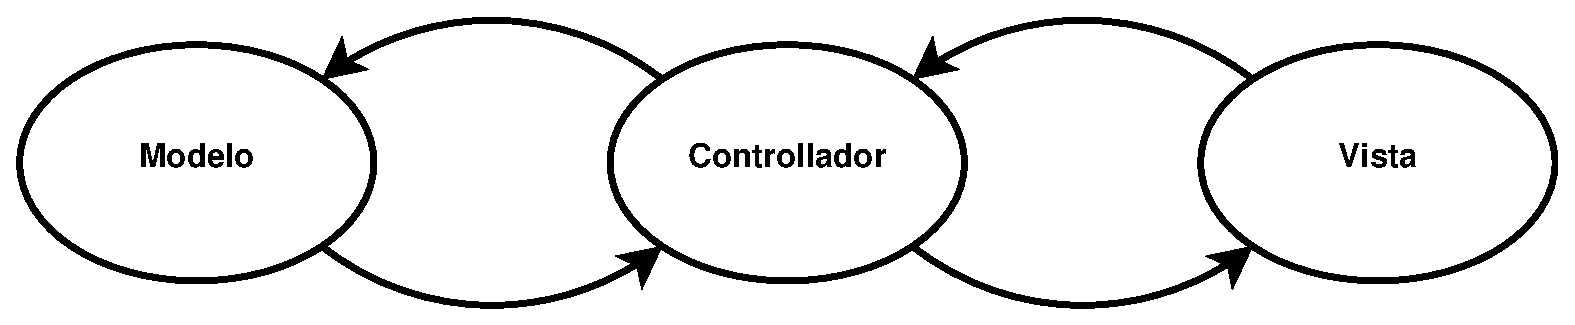
\includegraphics[scale=0.4]{dia-mvc-simple}
  \caption{Diagrama del patrón MVC\cite{JavaDesignPatternsExamples}.}
  \label{fig:dia-mvc-simple}
\end{figure}

%\section{Inversión de control}\label{sec-ioc}
%\textcolor{blue}{Vale por la descripción de inversión de control.}

%\section{Inyección de dependencia}\label{sec-dep-inj}
%\textcolor{blue}{Vale por la descripción de inyección de dependencia.}

\iffalse
%\section{Arquitectura 4+1} Organiza cada decisión en el diseño del sistema en cuatro partes llamadas vistas (ver Figura \ref{fig:dia-arq-4-1}), cada vista se encarga de enfocarse en un aspecto del diseño, estas cuatro vistas son unificadas por una cuarta vista de escenarios o casos de uso\cite{ViewModel4plus1}:
%\begin{itemize}
%	\item \textbf{Vista Lógica}: son las reglas del negocio por las que se rige la operación del usuario final.
%	\item \textbf{Vista de Proceso}: refleja concurrencia y sincronización.
%	\item \textbf{Vista de Física}: describe las relaciones del software con el hardware.
%	\item \textbf{Vista de Desarrollo}: describe la organización estática del software en su ambiente de desarrollo.
%\end{itemize}
%
%\begin{figure}[h]
%\centering
%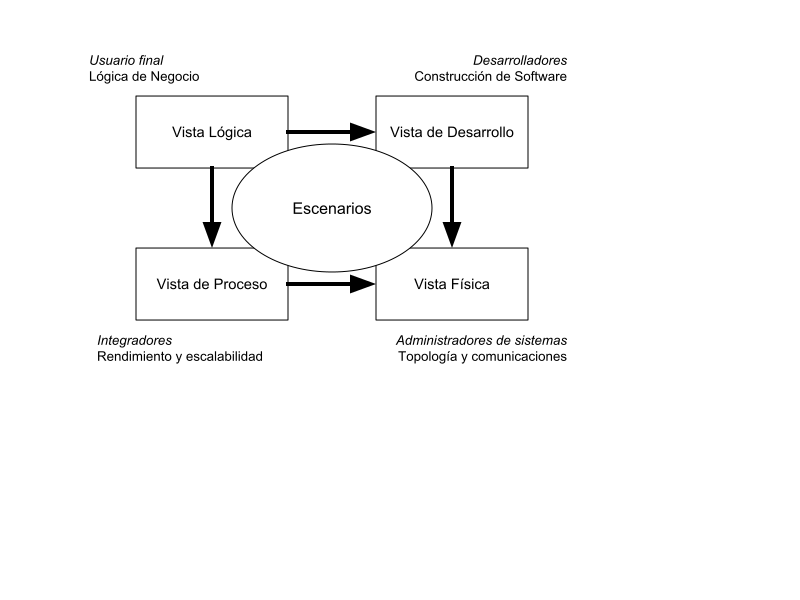
\includegraphics[scale=0.5]{dia-arq-4-1} 
%\caption{Diagrama de arquitectura 4+1.\cite{ViewModel4plus1}}
%\label{fig:dia-arq-4-1}
%\end{figure}
%
%
%\section{Arquitectura Orientada a Servicios}
%Thomas Erl describe la Arquitectura Orientada a Servicios (\textbf{SOA} por sus siglas en inglés) como el modelo arquitectónico del cómputo orientado a servicios\cite{SOAWithRest}, a continuación se muestran las definiciones de Erl sobre los conceptos de Orientación a Servicios:
%\begin{quote}
%La \textbf{Orientación a Servicios} es el paradigma de diseño dedicado para la creación de unidades lógicas de solución que son moldeados individualmente para que puedan ser utilizados colectiva y repetidamente para la realización de objetivos estratégicos y beneficios asociados con el cómputo orientado a servicios.\\
%El \textbf{Cómputo Orientado a Servicios} es engloba distintas plataformas de cómputo distribuido. En sí envuelve su propio paradigma y principios de diseño, catálogos de diseño de patrones, lenguajes, modelo arquitectónico junto con sus conceptos relacionados, tecnologías y marcos de trabajo.\\
%La \textbf{Arquitectura Orientada a Servicios} es un modelo de tecnología arquitectónica para soluciones orientadas a servicios con distintas características en apoyo de realizar orientación a servicios y los objetivos estratégicos asociados con el cómputo orientado a servicios.\cite{SOAWithRest}
%\end{quote}
\fi